\section{2D variations}

\begin{frame}{2 dimensional variations}
	\begin{block}{}
		We can vary the rules and space of two-dimensional cellular automata in
		multiple ways:
		\begin{itemize}
			\only<+->{\item different tilings (triangles, hexagons, penrose \dots),}
			\only<+->{\item more states (usually denoted with colors),}	%	already said?
			\only<+->{\item accounting for different positions,}
			\only<+(-1)->{\item \dots.}
		\end{itemize}
	\end{block}
	\only<1>{\begin{center}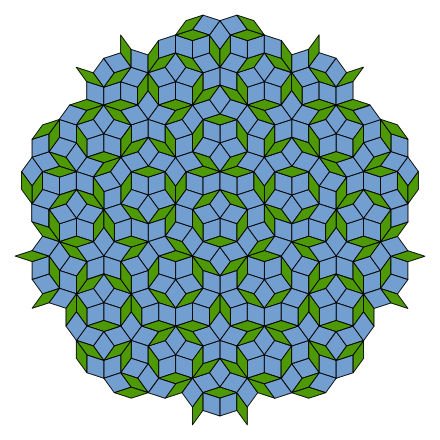
\includegraphics[width=.4\textwidth]{penrose_tiling.png}\end{center}}
\end{frame}

\section{Life}

\begin{frame}{The Game of Life}
	\begin{block}{Conway's Game of Life}<+->
		In 1970 John Horton Conway devised \textit{The Game of Life}, which is
		played in a 2-dimensional grid with two possible states for each cell, with
		the rules:
		\begin{enumerate}
			\item<+-> Every dead cell with exactly \( 3 \) live neighbours becomes alive,
			otherwise it stays dead.
			\item<+-> Every live cell with exactly \( 2 \) or \( 3 \) live neighbours
			stays alive, otherwise it dies.
		\end{enumerate}
	\end{block}

	\begin{block}{Rule string notation}<+->
		B3/S23 (B - born, S - survives)	%	TODO reword
	\end{block}
\end{frame}

\begin{frame}{Common constructs in Life}
	\only<+>{
		\begin{block}{Still lifes}
			Retain their shape through generations.
		\end{block}
		\begin{center}
			%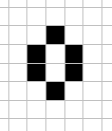
\includegraphics[width=0.2\textwidth]{still_beehive.png}
			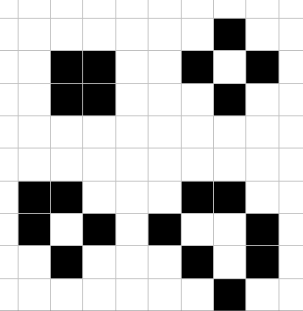
\includegraphics[width=0.4\textwidth]{stills.png}
		\end{center}
	}

	\only<2-3>{
		\begin{block}{Oscillators}
			Loop through a finite number of states and stays in the same location.
		\end{block}
		\begin{center}
			\only<2>{
				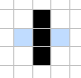
\includegraphics[width=0.3\textwidth]{oscilator_bar.png}
				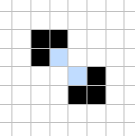
\includegraphics[width=0.3\textwidth]{oscilator_blocks.png}
			}

			\only<3>{
				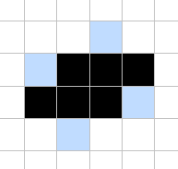
\includegraphics[width=0.3\textwidth]{oscilator_toad3.png}
				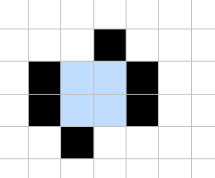
\includegraphics[width=0.3\textwidth]{oscilator_toad2.png}
			}
		\end{center}
	}

	\only<+(2)->{
		\begin{block}{Spaceships}
			Loop through a finite number of states and moves across the field. The most
			notable one is the glider.
		\end{block}

		\begin{center}
			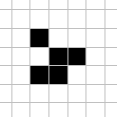
\includegraphics[width=0.17\textwidth]{glider_1.png}
			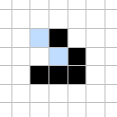
\includegraphics[width=0.17\textwidth]{glider_2.png}
			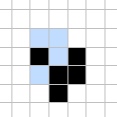
\includegraphics[width=0.17\textwidth]{glider_3.png}
			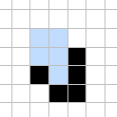
\includegraphics[width=0.17\textwidth]{glider_4.png}
			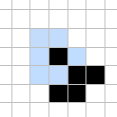
\includegraphics[width=0.17\textwidth]{glider_5.png}
		\end{center}

		\begin{center}
			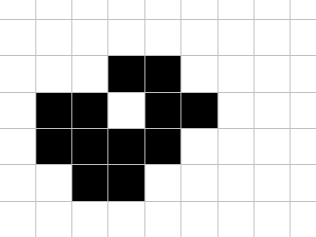
\includegraphics[width=0.17\textwidth]{spaceship_1.png}
			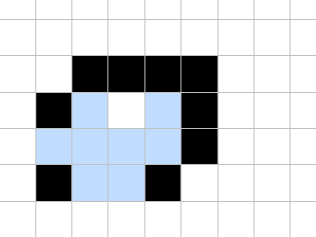
\includegraphics[width=0.17\textwidth]{spaceship_2.png}
			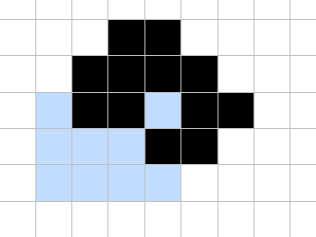
\includegraphics[width=0.17\textwidth]{spaceship_3.png}
			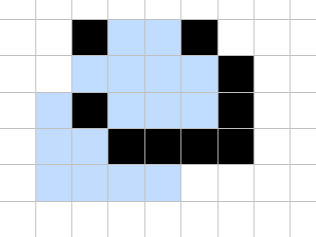
\includegraphics[width=0.17\textwidth]{spaceship_4.png}
			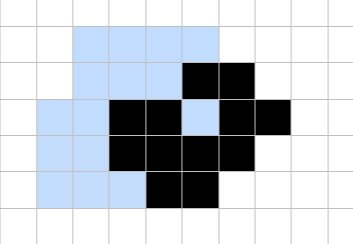
\includegraphics[width=0.17\textwidth]{spaceship_5.png}
		\end{center}
	}

\end{frame}
